\documentclass[border=2pt]{standalone}
\usepackage{pgfplots}
\begin{document}
	
    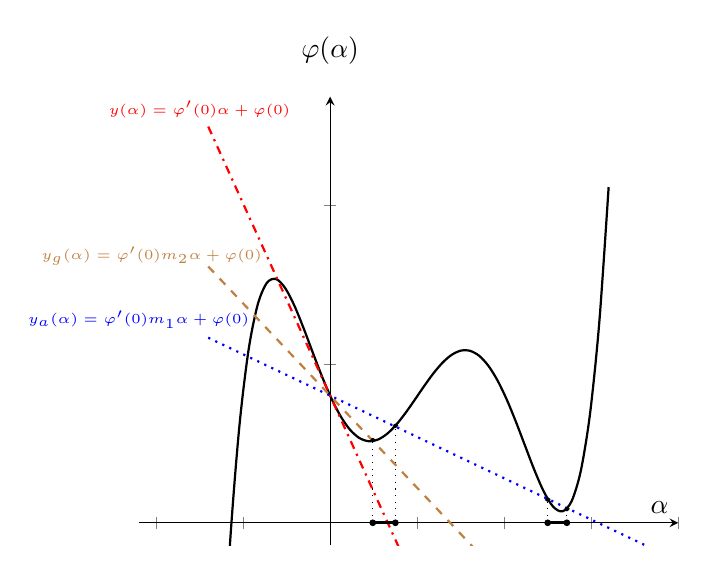
\begin{tikzpicture}[declare function={
    	f(\x)=0.988*\x^5-4.96*\x^4+4.978*x^3+5.015*x^2-6.043*x+4;
    	df(\x)=-6.043*\x +4;
    	a(\x) = -1.3*\x + 4;
    	g(\x) = -2.9*\x + 4;
    	i(\x) = 0;}]
        \begin{axis}[
            % center the x axis
            axis x line=middle,
            % we don't need a y axis line ...
            axis y line=middle,
            % ... and thus there is no need for much `height' of the axis
            %height=150pt,
            % but `height' also changes `width' which is restored here
            %width=\axisdefaultwidth,
            xmin=-2.2,
            xmax=4,
            ymin=-0.7,
            ymax=13.4,
            ylabel style={rotate=-90},
            xticklabels={,,},
            yticklabels={,,},
            xlabel={$\alpha$},
            ylabel={$\varphi(\alpha)$},
            samples=50,
            every axis y label/.style={
            	at={(ticklabel* cs:1.05)},
            	anchor=south,
            }
        ]
        
	  \addplot[domain=-2:3.2,thick,smooth] (x,{f(x)});
	  
	  \addplot[domain=-1.4:4.2,thick,dashdotted,red] (x,{df(x)});
	  \addplot[mark=text, mark options={fill=red}, text mark={\tiny $y(\alpha) = \varphi'(0)\alpha + \varphi(0)$}] coordinates {(-1.5, 13)};
	  
	  \addplot[domain=-1.4:4.2,thick,dotted, blue] (x,{a(x)});
	  \addplot[mark=text, mark options={fill=blue}, text mark={\tiny $y_{\tiny a}(\alpha) = \varphi'(0) m_1\alpha + \varphi(0)$}] coordinates {(-2.2, 6.4)};
	  
	  \addplot[domain=-1.4:4.2,thick,dashed, brown] (x,{g(x)});
	  \addplot[mark=text, mark options={fill=brown}, text mark={\tiny $y_{\tiny g}(\alpha) = \varphi'(0) m_2\alpha + \varphi(0)$}] coordinates {(-2.05, 8.4)};
      
	\addplot[domain=0.49:0.75, very thick] (x, {i(x)});
	\addplot[mark=*,mark size=1,mark options={fill=black}] coordinates {(0.49, 0)} node{};
	\addplot[mark=*,mark size=.8,mark options={fill=black},dotted] coordinates {(0.49, 0) (0.49, 2.6)} node{};
	\addplot[mark=*,mark size=1,mark options={fill=black}] coordinates {(0.75,0)} node{};
	\addplot[mark=*,mark size=.8,mark options={fill=black},dotted] coordinates {(0.75, 0) (0.75, 3.05)} node{};
	
	\addplot[domain=2.5:2.72, very thick] (x, {i(x)});
	\addplot[mark=*,mark size=1,mark options={fill=black}] coordinates {(2.5, 0)} node{};
	\addplot[mark=*,mark size=.8,mark options={fill=black},dotted] coordinates {(2.5, 0) (2.5, .73)} node{};
	\addplot[mark=*,mark size=1,mark options={fill=black}] coordinates {(2.72,0)} node{};
	\addplot[mark=*,mark size=.8,mark options={fill=black},dotted] coordinates {(2.72, 0) (2.72, .43)} node{};
	
    
        \end{axis}
    \end{tikzpicture}
\end{document}